\renewcommand{\thislecture}{3 }

%
% Cover page
%

\title[Neutrino Physics / Lecture \thislecture]
{
  {\huge \color{yellow} Neutrino Physics - Lecture \thislecture} \\
  {\it Oscillations at the Atmospheric Squared-Mass Splitting:\\Discovery and Current Status}\\
}

\author[C.Andreopoulos] {
  Professor Costas Andreopoulos\inst{1,2}
}
\institute[Liverpool/STFC-RAL] {
   \inst{1} University of Liverpool,
   \inst{2} STFC Rutherford Appleton Laboratory\\
   \vspace{0.5cm}
   {\it {\color{magenta} A post-graduate student lecture course}}\\
   \vspace{0.2cm}
}
\date{\today}

\titlegraphic{
  \includegraphics[height=25px]{./images/logo/liverpool.png}
  \hspace{3px}
  \includegraphics[height=30px]{./images/logo/ral.png}
}

	



\begin{frame}[plain]
  \titlepage
\end{frame}

%
% Outline
%

\begin{frame}{Outline for Lecture \thislecture}

\begin{itemize}
{\scriptsize
  \item Atmospheric neutrinos and atmospheric neutrino flux
  \item Interactions of atmospheric neutrinos
  \item First detection of atmospheric neutrinos: East Rand / Kolar Gold Field
  \item Revived interest: Atmospheric neutrinos as background to nucleon decay
  \item The atmospheric neutrino anomaly
  \item Explaining the anomaly: 1998 Super-Kamiokande observation
  \item Super-Kamiokande L/E analysis
  \item Confirmation with accelerator neutrinos
  \item Two-detector long-baseline neutrino oscillation paradigm
  \item K2K and MINOS
  \item $\nu_{\mu} \rightarrow \nu_{\tau}$ searches at Super-Kamiokande and OPERA
  \item Searches for subdominant oscillations - $\theta_{13}$ gateway to CPV
  \item First $\nu_{\mu} \rightarrow \nu_{e}$ results by T2K and MINOS
  \item Precision $\theta_{13}$ measurement by reactor experiments
  \item Accelerator experiment (T2K, NOvA) evidence for CPV and MO\\
}
\end{itemize}


\end{frame}

%
%
%

\begin{frame}[t]{Atmospheric neutrinos}

{\small
\centering
Neutrinos produced from interactions of cosmic rays with the atmosphere.\\
}
%\begin{center}
\vspace{0.1cm}
\begin{columns}
  \begin{column}{0.64\textwidth}
    \begin{minipage}{0.48\linewidth}
       \includegraphics[width=0.99\textwidth]{./images/3nu/atmo/flux_schematic.png}\\
    \end{minipage}\hfill
    \begin{minipage}{0.48\linewidth}
       \begin{itemize}
       {\scriptsize
         \item Neutrinos energies from $\sim$100 MeV to more than $\sim$100 TeV
         \item Flight paths from $\sim$10 km to $\sim$13,000 km\\
       }
       \end{itemize}
    \end{minipage}
    \includegraphics[width=0.99\textwidth]{./images/3nu/atmo/flux_energy_spectrum_and_ratio.png}
  \end{column}
  \begin{column}{0.35\textwidth}
   {\small
     Flux characteristics:
      \begin{itemize}
        \item $\sim$10\% uncertainties $<$10 GeV, much higher at higher energy
        \item Up/down symmetric above a few GeV
        \item $\nu_{\mu}/\nu_{e}$ ratio accurately known
              ($\sim$3\% in the $\sim$few GeV range)
         \item $\nu/\bar{\nu}$ ratio also accurately known
      \end{itemize}
   }
  \end{column}
\end{columns}
\end{frame}


\begin{frame}{Neutrino interactions in the $\sim$GeV energy range}
\centering
\includegraphics[width=0.85\textwidth]{./images/etc/vNxsec.png}\\
\begin{columns}
  \begin{column}{0.33\textwidth}
    \includegraphics[width=0.95\textwidth]{./images/etc/qe.png}
  \end{column}
  \begin{column}{0.33\textwidth}
    \includegraphics[width=0.95\textwidth]{./images/etc/res.png}
  \end{column}
  \begin{column}{0.33\textwidth}
    \includegraphics[width=0.95\textwidth]{./images/etc/dis.png}
  \end{column}
\end{columns}
\end{frame}



\begin{frame}[t]{Detection of atmospheric neutrinos}

\begin{columns}
  \begin{column}{0.38\textwidth}
       \begin{itemize}
          {\scriptsize
            \item First atmospheric neutrino detection in 1965 nearly
              simultaneously by 2 experiments.
            \item In the East Rand gold mine (3.2 km depth) in South
                      Africa using a liquid scintillator detector
                      {\scriptsize \color{blue} [Reines et al, Phys.Rev.Lett. 15 (1965) 429}
            \item In the Kolar
                      Gold Field mine (2.4 km depth) using a plastic
                      scintillator detector
                      {\scriptsize \color{blue} [Achar et al, Phys.Lett. 18
                        (1965) 196}\\
            \item Primary motivation to investigate weak interactions
                      at high energies.
            \item Predicted/Observed = 1.6 $\pm$ 0.4
                      {\scriptsize \color{blue} [Crouch et al, Phys.Rev. D18
                        (1978) 2239}\\

           }
       \end{itemize}
  \end{column}
  \begin{column}{0.62\textwidth}
     \centering
      \includegraphics[width=0.99\textwidth]{./images/3nu/atmo/first_obs_abstract.png}\\
      \includegraphics[width=0.80\textwidth]{./images/3nu/atmo/first_obs_zenith.png}\\
  \end{column}
\end{columns}
\end{frame}


\begin{frame}[t]{Atmospheric neutrinos as background to proton decay}
\begin{columns}[t]
  \begin{column}{0.50\textwidth}
   \begin{itemize}
    {\small
     \item In the 80's the interest for atmospheric neutrinos was revived.\\
           \vspace{0.4cm}
     \item Grand Unified Theories (GUTs) predicted that the proton might be unstable
           and several experimental searches (using fine-grained tracking or water
           Cherenkov detectors) were conducted [IMB, Kamiokande, Soudan, NUSEX]\\
           \vspace{0.4cm}
     \item Interactions of atmospheric neutrinos were a background to proton decay
           searches, so atmospheric neutrinos were studied.
    }
   \end{itemize}
  \end{column}
  \begin{column}{0.50\textwidth}
   {\small
    \centering
    These studies found the $\nu_{\mu}/\nu_{e}$ ratio to be significantly lower than expected (with good accuracy).\\
    \vspace{0.2cm}
    This was puzzling and became known as the {\em \color{red} atmospheric neutrino anomaly.}\\
    \vspace{0.4cm}
    \includegraphics[width=0.90\textwidth]{./images/3nu/atmo/dblratio.png}\\
   }
  \end{column}
\end{columns}
\end{frame}

%
%
%

\begin{frame}{The Super-Kamiokande experiment}
\begin{columns}
 \begin{column}{0.45\textwidth}
    \includegraphics[height=0.85\textheight]{./images/3nu/atmo/superk_inside_view_portrait_1.jpg}
 \end{column}
 \begin{column}{0.55\textwidth}
 {\small
 \begin{itemize}
   \item 50 kt Water Cherenkov detector\\ (22.5 kton fiducial)
   \item Overburden (shielding): 2700 mwe
   \item Inner Detector (ID): 11,129 20'' PMTs\\ (40\% photo-cathode coverage)
   \item Outer Detector (OD): 1,885 8'' PMTs
   \item Energy threshold: $\sim$ 4.5 MeV
 \end{itemize}
 }
 \end{column}
\end{columns}
\end{frame}

%
%
%

\begin{frame}{Water Cherenkov Imaging}

\begin{columns}
  \begin{column}{0.70\textwidth}
    \begin{center}
    \includegraphics[width=0.45\textwidth,height=0.40\textheight]{./images/3nu/atmo/superk_1Rmu.png}
    \includegraphics[width=0.45\textwidth,height=0.40\textheight]{./images/3nu/atmo/superk_1Re.png}\\
   \end{center}
  \end{column}
  \begin{column}{0.30\textwidth}
    \centering
    {\scriptsize
      Cherenkov cone opening angle: {\color{red}$cos\theta=1/{\beta}n$}\\
      \vspace{0.2cm}
      In water (refractive index n=1.33) and for
      a highly relativistic particle: {\color{red} $\theta=42$ degrees}\\
    }
  \end{column}
\end{columns}
\begin{columns}
  \begin{column}{0.65\textwidth}
    \centering
    \vspace{0.3cm}
    {\bf $\mu$-like and e-like event topologies identified based on the Cherenov ring pattern.}\\
    \vspace{0.2cm}
    Mis-ID probability below 1GeV/c is $<$1\%.
  \end{column}
  \begin{column}{0.35\textwidth}
    \includegraphics[width=0.95\textwidth]{./images/3nu/atmo/sk_pid.png}\\
  \end{column}
\end{columns}
\end{frame}


\begin{frame}[t]{SK atmospheric neutrino measurement (1998)}

\begin{columns}
  \begin{column}{0.50\textwidth}
   {
    \centering
    \includegraphics[width=0.85\textwidth]{./images/3nu/atmo/up_down_schematic.png}\\
   }
   {\scriptsize
    For downward-going neutrinos the flight length is $\sim$20 km whereas
    for upward-going ones is $\sim$ 13,000 km.\\
    For ${\Delta}m^{2}\sim$10$^{-3}$ $eV^{2}/c^{4}$ the oscillation length is of the order
    of few hundred km, then for upward-going neutrinos the oscillation effect is averaged out.\\
    The up/down ratio is $\sim$ 1 - 0.5 $\cdot$ $sin^{2}2\theta_{23}$\\
   }
  \end{column}
  \begin{column}{0.50\textwidth}
    \includegraphics[width=0.92\textwidth]{./images/3nu/atmo/sk_zenith_1998.png}
  \end{column}
\end{columns}
\end{frame}


\begin{frame}[t]{SK atmospheric neutrino measurement (2014)}

\begin{columns}
  \begin{column}{0.30\textwidth}
    \includegraphics[width=0.95\textwidth]{./images/3nu/atmo/sk_event_categories.png}
  \end{column}
  \begin{column}{0.70\textwidth}
    {\scriptsize
      19 analysis samples analysis included in latest analysis\\
      Due to the wide range of energies and baselines and the high statistics,
      atmospheric neutrinos are a fantastic tool complementing the accelerator searches $\rightarrow$
      sensitivity to subleading effects.\\
    }
    \includegraphics[width=0.95\textwidth]{./images/3nu/atmo/sk_zenith_2014.png}
  \end{column}
\end{columns}
{\scriptsize \color{blue}[Wendell, Neutrino 2014 conference, Boston]}
\end{frame}


\begin{frame}[t]{SK atmospheric neutrino L/E analysis}
\centering
{\bf Neutrino oscillations ($\pbar{\nu}_{\mu} \rightarrow \pbar{\nu}_{\tau}$) describe the atmospheric data well.}\\
However, alternative models were also proposed.\\
\vspace{0.2cm}
\begin{columns}
  \begin{column}{0.50\textwidth}
    \centering
    {\scriptsize
     {\bf The smoking-gun signature for neutrino oscillations is ..., well, {\em oscillations}}.\\
     To be confident for the observation of oscillations we need to see wiggles.\\
    }
    \includegraphics[width=0.80\textwidth]{./images/3nu/atmo/le_schematic.png}\\
    {\scriptsize {\color{blue}[oscillations]} {\color{red}[decoherence]} {\color{green}[decay]}}
  \end{column}
  \begin{column}{0.50\textwidth}
    \centering
    {\scriptsize
      3903 days of SK atmospheric data.\\
      Decay (decoherence) disfavoured at 4$\sigma$ (4.8$\sigma$).\\
    }
    \includegraphics[width=0.90\textwidth]{./images/3nu/atmo/sk_le.png}\\
    {\scriptsize \color{blue}[Wendell, Neutrino 2014 conference, Boston]}
  \end{column}
\end{columns}
\end{frame}

%
%
%

\begin{frame}[t]{Confirmation with accelerator neutrinos}

\begin{itemize}
  {\small
  \item The atmospheric neutrino result was {\em very} convincing\\
  \item The data suggested $\pbar{\nu}_{\mu}$ oscillations with
     \begin{itemize}
     {\small
         \vspace{0.2cm}
         \item nearly maximal mixing ({\color{red}$\theta_{23} \approx 45^{o}$}), and
         \vspace{0.2cm}
         \item {\color{red} $|{\Delta}m^{2}_{32}| \approx 2.5 \times 10^{-3} eV^{2}/c^{4}$}.
     }
     \end{itemize}
     \vspace{0.3cm}
  \item But {\bf confirmation} and, subsequently, {\bf precision measurements} were needed in
        a {\bf controlled environment with a man-made beam}
  \vspace{0.3cm}
  \item The measured value of $|{\Delta}m^{2}_{32}|$ suggested an appropriate baseline
     \begin{itemize}
        {\small
         \vspace{0.2cm}
         \item L (km) $\approx$ $\frac{\pi}{2 \cdot 1.267} \cdot
                 \frac{E_{\nu} (GeV)}{|{\Delta}m^{2}_{32}| (eV^{2}/c^{4})}$
         \vspace{0.2cm}
         \item For $E_{\nu}$ = O(1 GeV) and
               $|{\Delta}m^{2}_{32}|$ = O($10^{-3} eV^{2}/c^{4}$),
               L $\approx$ O($10^{3}$ km)!
        }
     \end{itemize}
  }
\end{itemize}
\end{frame}

%
%
%

\begin{frame}[t]{Confirmation with accelerator neutrinos}

Confirmation with accelerator neutrinos was {\bf challenging}!!\\
\vspace{0.2cm}
Besides the technical difficulties making of a $\nu$ beam and pointing it several
hunderds of km away to a massive underground detector, there were
{\bf substantial uncertainties} in our understanding of
\begin{itemize}
{\small
\item accelerator-made neutrino beam fluxes, and
\item few-GeV neutrino scattering of nuclear targets
}
\end{itemize}

Hence the emergence of the {\bf two-detector}
long-baseline experiments\\
\begin{center}
\includegraphics[width=0.95\textwidth]{./images/3nu/accelerator/two_detector.png}\\
\end{center}

\end{frame}

%
%
%

\begin{frame}[t]{Two-detector experiments}

  \begin{center}
  \includegraphics[width=0.95\textwidth]{./images/3nu/accelerator/two_detector_extrapolation_simple.png}\\
  \end{center}

\end{frame}

%
%
%

\begin{frame}[t]{How to make a (conventional) neutrino beam}

\begin{columns}
  \begin{column}{0.78\textwidth}
    \centering
    \includegraphics[width=0.95\textwidth]{./images/3nu/accelerator/numi.png}\\
    \vspace{0.2cm}
    \includegraphics[width=0.32\textwidth]{./images/3nu/accelerator/beam_horn_old_1.jpg}
    \hfill
    \includegraphics[width=0.66\textwidth]{./images/3nu/accelerator/beam_horn_old_3.jpg}
  \end{column}
  \begin{column}{0.22\textwidth}
   \begin{block}{}
   {\scriptsize
    Where do our $\nu$'s come from?\\
    \vspace{0.3cm}
    $\pi^{+} \rightarrow {\color{red}\nu_{\mu}} + \mu^{+}$\\
    $\pi^{-} \rightarrow {\color{magenta}\bar{\nu}_{\mu}} + \mu^{-}$\\
    $\mu^{+} \rightarrow {\color{magenta}\bar{\nu}_{\mu}} + {\color{blue}\nu_{e}} + e^{+}$\\
    $\mu^{-} \rightarrow {\color{green}\bar{\nu}_{e}} + {\color{red}\nu_{\mu}} + e^{-}$\\
    $K^{+} \rightarrow {\color{red}\nu_{\mu}} + \mu^{+}$\\
    $K^{+} \rightarrow {\color{blue}\nu_{e}} + \pi^{0} + e^{+}$\\
    $K^{+} \rightarrow {\color{red}\nu_{\mu}} + \pi^{0} + \mu^{+}$\\
    $K^{-} \rightarrow {\color{magenta}\bar{\nu}_{\mu}} + \mu^{-}$\\
    $K^{-} \rightarrow {\color{green}\bar{\nu}_{e}} + \pi^{0} + e^{-}$\\
    $K^{-} \rightarrow {\color{magenta}\bar{\nu}_{\mu}} + \pi^{0} + \mu^{-}$\\
    $K_{L}^{0} \rightarrow {\color{magenta}\bar{\nu}_{\mu}} + \pi^{+} + \mu^{-}$\\
    $K_{L}^{0} \rightarrow {\color{red}\nu_{\mu}} + \pi^{-} + \mu^{+}$\\
    $K_{L}^{0} \rightarrow {\color{green}\bar{\nu}_{e}} + \pi^{+} + e^{-}$\\
    $K_{L}^{0} \rightarrow {\color{blue}\nu_{e}} + \pi^{-} + e^{+}$\\
  }
  \end{block}
  \end{column}
\end{columns}
\end{frame}


\begin{frame}[t]{Confirmation with accelerator neutrinos: K2K and MINOS}

\begin{columns}
  \begin{column}{0.40\textwidth}
    \includegraphics[width=0.99\textwidth]{./images/3nu/accelerator/k2k_layout.png}
  \end{column}
  \begin{column}{0.60\textwidth}
    \begin{itemize}
    {\scriptsize
      \item K2K (KEK to Kamioka, 250km), 06/1999-11/2004\\
      \item Using a $\nu_{\mu}$ beam made at the KEK 12-GeV proton synchrotron (peak $E_{\nu}$ $\approx$ 1 GeV)
      \item Used 50-kt Super-K as far detector
      \item Near detectors at $\sim$300m from the target: 1kt water Cherenkov + fine-grained tracking detectors\\
    }
    \end{itemize}
  \end{column}
\end{columns}

\begin{columns}
  \begin{column}{0.45\textwidth}
    \begin{itemize}
    {\scriptsize
      \item MINOS (FNAL to Soudan, 735 km), 2005-2018\\
      \item Using a $\pbar{\nu}_{\mu}$ beam made at the 120-GeV Main Injector at FNAL (several beam configurations:
            peak $E_{\nu}$ $\approx$ 3.5-8 GeV)
      \item 5.4 kt steel-scintillator magnetized tracking calorimeter 0.7km underground
      \item 1-kt steel-scintillator magnetized tracking calorimeter near detector, $\sim$1km the from source and 100m underground\\
    }
    \end{itemize}
  \end{column}
  \begin{column}{0.25\textwidth}
    \includegraphics[width=0.99\textwidth]{./images/3nu/accelerator/minos_layout_2.jpg}
  \end{column}
  \begin{column}{0.30\textwidth}
    \includegraphics[width=0.99\textwidth]{./images/3nu/accelerator/minos_far_det.png}
  \end{column}
\end{columns}
\end{frame}


\begin{frame}[t]{MINOS detector}
  \begin{center}
  \includegraphics[width=0.80\textwidth]{./images/3nu/accelerator/minos_detector_01.png}\\
  \end{center}
\end{frame}

\begin{frame}[t]{MINOS detector}

  {\scriptsize
   Massive segmented iron calorimeters, with inexpensively produced plastic scintillator
   as active material. The scintillation light is collected by WLS fibers read out by
   multi-anode PMTs.\\
  }
  \begin{center}
  \includegraphics[width=0.75\textwidth]{./images/3nu/accelerator/minos_detector_02.png}\\
  \end{center}
\end{frame}

\begin{frame}[t]{MINOS detector: A feat of engineering}
  \begin{center}
  \includegraphics[width=0.90\textwidth]{./images/3nu/accelerator/minos_detector_03.png}\\
  \end{center}
\end{frame}


\begin{frame}[t]{MINOS event topologies}
  \begin{center}
  \includegraphics[width=0.95\textwidth]{./images/3nu/accelerator/minos_events.png}\\
  \end{center}
\end{frame}


\begin{frame}[t]{MINOS came close to being the wrong experiment}
  \begin{center}
  \includegraphics[width=0.95\textwidth]{./images/3nu/accelerator/minos_wrong_dmsq.png}\\
  \end{center}
\end{frame}

\begin{frame}[t]{MINOS - Saved by its tunable neutrino beam}
  \begin{center}
  \includegraphics[width=0.95\textwidth]{./images/3nu/accelerator/minos_tunable_beam.png}\\
  \end{center}
\end{frame}


\begin{frame}[t]{K2K and MINOS $\pbar{\nu}_{\mu}$ disappearance results}

\begin{columns}
  \begin{column}{0.41\textwidth}
    \begin{itemize}
    {\scriptsize
      \item {\bf K2K:} Analyzed 0.92$\times10^{20}$ POT.
      \item 158.1$^{+9.2}_{8.6}$ events were expected with no oscillations, but only 112 were seen.
      \item Out of those events, the energy could be reconstructed for 58 1-ring $\mu$-like events
            and energy distrortions were seen.
      \item No oscillation excluded at 4.3$\sigma$.\\
    }
    \end{itemize}
    {\centering
      \includegraphics[width=0.70\textwidth]{./images/3nu/accelerator/k2k_spectrum.png}\\
      {\scriptsize \color{blue}[PRD 74 (2006), 072003]}\\
    }
  \end{column}
  \begin{column}{0.59\textwidth}
    \begin{itemize}
    {\scriptsize
      \item {\bf MINOS:} Analyzed 10.71$\times10^{20}$ POT in a $\nu_{\mu}$ beam and
            3.36$\times10^{20}$ POT in a $\bar{\nu}_{\mu}$-enhanced beam
      \item Jointly with atmospheric $\nu$ sample (48.67 kt$\cdot$yr)
      \item High statistics / precision measurements\\
    }
    \end{itemize}
    {\centering
      \includegraphics[width=0.80\textwidth]{./images/3nu/accelerator/minos_disapp_spectra.png}\\
      {\scriptsize \color{blue}[Sousa, Neutrino 2014, Boston]}\\
    }
  \end{column}
\end{columns}
\end{frame}


\begin{frame}[t]{K2K and MINOS $\pbar{\nu}_{\mu}$ disappearance results}

  \begin{columns}
    \begin{column}{0.60\textwidth}
      {\centering
        \includegraphics[width=0.95\textwidth]{./images/3nu/accelerator/minos_disapp_cont_2011.png}\\
        {\scriptsize \color{blue}[PRL 106 (2011), 181801]}\\
      }
    \end{column}
    \begin{column}{0.40\textwidth}
      MINOS ushered the atmospheric sector into the "precision era" [*].\\
      \vspace{2.5cm}
      {\small
        [*] We no longer had to draw confidence regions in log scale.
      }
    \end{column}
  \end{columns}

\end{frame}


\begin{frame}[plain,c]
 \begin{center}
 {\Large
  {\bf So, $\nu_{\mu}$'s oscillate away.\\ But what do they oscillate to?\\}
 }
 \end{center}
 \vspace{0.3cm}
 We knew for the Super-Kamiokande atmospheric measurement that
 $\nu_{\mu} \rightarrow \nu_{e}$ was not the dominant mode.\\
 \vspace{0.3cm}
 This leaves two obvious possibilities:
 \begin{itemize}
         \item $\nu_{\mu} \rightarrow \nu_{\tau}$
         \item $\nu_{\mu} \rightarrow \nu_{sterile}$
 \end{itemize}
\end{frame}


\begin{frame}[t]{Search for $\nu_{\tau}$ at Super-Kamiokande}

\begin{columns}
  \begin{column}{0.50\textwidth}
    \begin{itemize}
    {\small
     \item Expecting $\sim$ 1 (atmospheric) $\nu_{\tau}$ CC event per kt*year
     \item $\tau$ typically decays to hadrons (BR: $\sim$65\%) close to the primary interaction vertex ($<$ 1 mm)
     \item Complicated event topologies with several particles above Cherenkov threshold
     \item Difficult to separate from NC events on an event-by-event basis.
     \item But the number of $\nu_{\tau}$ induced by $\nu_{\mu}$ oscillations could be calculated statistically.
    }
    \end{itemize}
  \end{column}
  \begin{column}{0.50\textwidth}
    \centering
    \includegraphics[width=0.70\textwidth]{./images/3nu/atmo/nu_tau_reaction.png}\\
    \includegraphics[width=0.95\textwidth]{./images/3nu/atmo/sk_tau_display.png}\\
    $\nu_{\tau}$ event at SK (MC):\\
    {\scriptsize \color{blue}[Wendell, Neutrino 2014 conference, Boston]}
  \end{column}
\end{columns}
\end{frame}


\begin{frame}[t]{Search for $\nu_{\tau}$ at Super-Kamiokande}

\begin{columns}
  \begin{column}{0.47\textwidth}
    \includegraphics[width=0.95\textwidth]{./images/3nu/atmo/sk_tau_zenith.png}\\
    {\color{red} \small Neutrino-induced $\rightarrow$ Upward-going}\\
  \end{column}
  \begin{column}{0.53\textwidth}
     Statistical search for $\nu_{\tau}$ CC-like events using an exposure of 2,806 days\\
     \vspace{0.3cm}
     SK observed an event excess of:\\
     180.1 $\pm$ 44.3(stat) +17.8 -15.2 (syst)\\
     \vspace{0.3cm}
     The significance of this excess is 3.8$\sigma$\\
     \vspace{0.4cm}
     {\scriptsize \color{blue}[Wendell, Neutrino 2014 conference, Boston]}\\
     \noindent\rule{2cm}{0.4pt}\\
     {\small
        The atmospheric sample at Super-Kamiokande provides also a strong
        constraint on $\nu_{\mu} \rightarrow \nu_{sterile}$ oscillations
        by studying NC-enriched and upgoing $\mu$ samples.
     }
  \end{column}
\end{columns}
\end{frame}


%
% OPERA
%

\begin{frame}[t]{Direct search for $\nu_{\tau}$ CC interactions at OPERA}

{
\small
\centering
$\mu$m-scale resolution emulsion detector +
electronic spectrometer in Gran Sasso (3,800 mwe), at the CERN CNGS
$\nu_{\mu}$ beam ($<E_{\nu}> \approx$ 17 GeV) (2008-12)\\
}
\vspace{0.3cm}
\begin{columns}
  \begin{column}{0.40\textwidth}
   \centering
    {\small \color{red}
       $\nu_{\tau}$ CC interactions identified from the characteristic $\tau$ decay kink\\
    }
    \vspace{0.1cm}
    \includegraphics[width=0.90\textwidth]{./images/3nu/accelerator/opera_event_schematic.png}\\
    \includegraphics[width=0.98\textwidth]{./images/3nu/accelerator/opera_tau_1.png}
  \end{column}
  \begin{column}{0.60\textwidth}
    \centering
    \begin{itemize}
    {\small
     \item L/$<E_{\nu}> \approx$ 43 km/GeV: \\
           $P(\nu_{\mu} \rightarrow \nu_{e}) \approx$ 1\%\\
           ($\nu_{\tau}$ CC threshold = 3.5 GeV)
     \item Exposure of 1.797$\times$10$^{20}$ POT
     \item 10 $\nu_{\tau}$ CC events observed (expected background = 2 $\pm$ 0.4)
     \item $\nu_{\tau}$ appearance significance: 6.1$\sigma$
    }
    \end{itemize}
    \includegraphics[width=0.93\textwidth]{./images/3nu/accelerator/opera_tau_events_final.png}\\
    {\scriptsize \color{blue}[OPERA, Phys.Rev.Lett. 120 (2018) 21, 211801]}
  \end{column}
\end{columns}
\end{frame}

%
% \theta13 and subdominant osc
%

\begin{frame}[plain,c]
\begin{center}
{\Large
 So $\nu_{\mu}$'s oscillate predominantly to $\nu_{\tau}$\\
 \vspace{0.2cm}
 {\bf How about sub-dominant $\nu_{\mu}\rightarrow\nu_{e}$ oscillations}
}
\end{center}
\end{frame}

%
% init hints on \theta13
%

\begin{frame}[t]{$\theta_{13}$ a gateway to CPV}

\begin{center}
  \includegraphics[width=0.99\textwidth]{./images/3nu/accelerator/theta13_gateway_cpv_t2k_proposal.png}
\end{center}

\end{frame}


\begin{frame}{Initial hints for non-zero $\theta_{13}$}
\centering
For $\theta_{13}$=0, a small tension existed between the solar and
KamLAND values of $\theta_{12}$ (KamLAND favoured larger values).
\begin{columns}
  \begin{column}{0.50\textwidth}
     \includegraphics[width=0.99\textwidth]{./images/3nu/reactor/kamLAND_theta13_contour_v2.png}
  \end{column}
  \begin{column}{0.50\textwidth}
     \includegraphics[width=0.99\textwidth]{./images/3nu/reactor/kamLAND_theta13_projection.png}\\
     {\scriptsize \color{blue}[Phys. Rev. D 83, 052002 (2011)] and others}
  \end{column}
\end{columns}
\end{frame}

%
%
%

\begin{frame}{Two experimental strategies for measuring $\theta_{13}$}

\begin{itemize}
{\small
  \item {\bf $\bar{\nu}_{e}$ disappearance at short-baseline reactor experiments}\\
  \vspace{0.2cm}
  (Daya Bay, RENO, Double-Chooz)
  {\scriptsize
   \[
     \displaystyle
     P(\bar{\nu}_{e} \rightarrow \bar{\nu}_{e}) =
       1 - {\color{red}sin^{2}2\theta_{13}} \cdot sin^{2}(\frac{{\Delta}m^{2}_{ee} L}{4E_{\nu}})
         + (solar\;term)
%        - cos^{4}\theta_{13} \cdot sin^{2}2\theta_{12} \cdot sin^{2} (\frac{{\Delta}m^{2}_{21} L}{4E_{\nu}})
   \]
  }
  \item {\bf $\pbar{\nu}_{\mu} \rightarrow \pbar{\nu}_{e}$ appearance in
  long-baseline accelerator experiments}\\
  \vspace{0.2cm}
  ((MINOS,) T2K, NOvA)
  {\scriptsize
   \begin{eqnarray*}
%   \[
     \displaystyle
     P({\nu}_{\mu} \rightarrow {\nu}_{e})  & = &
         sin^{2}\theta_{23} \cdot {\color{red}sin^{2}2\theta_{13}} \cdot sin^{2}(\frac{{\Delta}m^{2}_{32} L}{4E_{\nu}}) \\
      & & - \frac{sin2\theta_{12} \cdot sin2\theta_{23} \cdot {\color{red}sin^{2}2\theta_{13}}}{2{\color{red}sin\theta_{13}}}
              \cdot sin^{2}(\frac{{\Delta}m^{2}_{21} L}{4E_{\nu}})
              \cdot sin^{2}(\frac{{\Delta}m^{2}_{32} L}{4E_{\nu}}) \cdot {\color{blue}sin\delta}  \\
      & & + (CP\;even\;term) + (matter\;effect\;term) + (solar\;term)
   \end{eqnarray*}
%   \]
  }
}
\end{itemize}
\end{frame}


\begin{frame}{The T2K experiment (2010-present)}
\begin{columns}
  \begin{column}{0.60\textwidth}
     \includegraphics[width=0.99\textwidth]{./images/3nu/accelerator/t2k_overview.png}
  \end{column}
  \begin{column}{0.40\textwidth}
  \begin{itemize}
  {\scriptsize
    \item Relatively pure $\nu_{\mu}$ ($\bar{\nu}_{\mu}$) beam.
    \item Produced using the 30-GeV proton beam at J-PARC
    \item Design power of 750 kW
    \item Near detectors: on-axis and off-axis at 280 m to monitor and constrain flux characteristics and interaction rates.
    \item Far detector: SuperK 50-kton (22.5 kton fiducial) water Cherenkov detector, 2.5 degrees off-axis, 295 km away.
    \item Neutrino flux at SuperK peaked at $\sim$0.6 GeV.
    \item L/E tuned to the `atmospheric' ${\Delta}m^{2}$ ($\sim$2.4$\times$10$^{-3}$ $eV^{2}/c^{4}$).
  }
  \end{itemize}
  \end{column}
\end{columns}
\end{frame}

%
%
%
\begin{frame}{T2K neutrino beam}

\begin{center}
  {\bf Primary proton beam from the 30-GeV J-PARC proton accelerator.}\\
\end{center}

\begin{columns}
  \begin{column}{0.75\textwidth}
     \includegraphics[width=0.99\textwidth]{./images/3nu/accelerator/t2k/jparc_facility_birds_eye_annotated.png}
  \end{column}
  \begin{column}{0.25\textwidth}
  \begin{itemize}
  {\scriptsize
    \item Fast extraction
    \item 8 bunches/spill
    \item 581 nsec bunch interval
    \item 58 nsec bunch width
    \item Rep. rate (May '16): 2.48 sec\\
    \item p/spill (May '16): 2.2$\times10^{14}$
    \item p/spill (design): 3.3$\times10^{14}$
    \item Power (May '16): 420 kW
    \item Power (design): 750 kW\\
  }
  \end{itemize}
  \end{column}
\end{columns}
\end{frame}

%
% The neutrino beamline
%
\begin{frame}{T2K neutrino beam}
\begin{columns}
  \begin{column}{0.78\textwidth}
   \begin{center}
    \includegraphics[width=0.99\textwidth]{./images/3nu/accelerator/t2k/neutrino_beamline_schematic.png}\\
   \end{center}
   \vspace{0.4cm}
   {\scriptsize
     {\bf Target:} A 2.6 cm wide, 91.4 cm (1.9 interaction lengths) long graphite rod \\
      %  (diameter: 2.6 cm, length: 91.4 cm / 1.9 interaction lengths).\\
     {\bf Focussing:}
       3 magnetic horns pulsed with 250 (max 320) kA currents generating $\sim$2 T field:
       $\sim$16$\times$ increase in $\nu$ flux w.r.t unfocussed beam.\\
     {\bf Decay volume:} A 96 m long steel decay tunnel\\
      %  (1.4 m (upstream) - 3.0 m (downstream) wide, 1.7 m - 5.0 m high).\\
   }
  \end{column}
  \begin{column}{0.22\textwidth}
   \begin{block}{}
   {\scriptsize
    Where do our $\nu$'s come from?\\
    \vspace{0.3cm}
    $\pi^{+} \rightarrow {\color{red}\nu_{\mu}} + \mu^{+}$\\
    $\pi^{-} \rightarrow {\color{magenta}\bar{\nu}_{\mu}} + \mu^{-}$\\
    $\mu^{+} \rightarrow {\color{magenta}\bar{\nu}_{\mu}} + {\color{blue}\nu_{e}} + e^{+}$\\
    $\mu^{-} \rightarrow {\color{green}\bar{\nu}_{e}} + {\color{red}\nu_{\mu}} + e^{-}$\\
    $K^{+} \rightarrow {\color{red}\nu_{\mu}} + \mu^{+}$\\
    $K^{+} \rightarrow {\color{blue}\nu_{e}} + \pi^{0} + e^{+}$\\
    $K^{+} \rightarrow {\color{red}\nu_{\mu}} + \pi^{0} + \mu^{+}$\\
    $K^{-} \rightarrow {\color{magenta}\bar{\nu}_{\mu}} + \mu^{-}$\\
    $K^{-} \rightarrow {\color{green}\bar{\nu}_{e}} + \pi^{0} + e^{-}$\\
    $K^{-} \rightarrow {\color{magenta}\bar{\nu}_{\mu}} + \pi^{0} + \mu^{-}$\\
    $K_{L}^{0} \rightarrow {\color{magenta}\bar{\nu}_{\mu}} + \pi^{+} + \mu^{-}$\\
    $K_{L}^{0} \rightarrow {\color{red}\nu_{\mu}} + \pi^{-} + \mu^{+}$\\
    $K_{L}^{0} \rightarrow {\color{green}\bar{\nu}_{e}} + \pi^{+} + e^{-}$\\
    $K_{L}^{0} \rightarrow {\color{blue}\nu_{e}} + \pi^{-} + e^{+}$\\
  }
  \end{block}
  \end{column}
\end{columns}
\end{frame}


\begin{frame}{Going {\em off-axis}}

{\bf T2K is the first accelerator experiment employing the {\em off-axis} trick.}

Exploits kinematical properties of pion decay to create a narrow-band neutrino beam
peaked at an energy chosen so as to maximize the oscillation probability at the SuperK location.

\begin{columns}
  \begin{column}{0.55\textwidth}
     \includegraphics[width=0.95\textwidth]{./images/3nu/accelerator/offaxis_angle_epi_vs_enu_degrees.png}
  \end{column}
  \begin{column}{0.45\textwidth}
     \includegraphics[width=0.80\textwidth]{./images/3nu/accelerator/oaeffect_flux.png}
  \end{column}
\end{columns}
\end{frame}


%
% Details about the off-axis beam
%
{
\setbeamercolor {frametitle}          {bg=dBG1}
\setbeamercolor {author in head/foot} {bg=dBG1}
\setbeamercolor {title in head/foot}  {bg=dBG2}
\setbeamercolor {date in head/foot}   {bg=dBG3}
\setbeamercolor {date in head/foot}   {fg=dFG3}

\begin{frame}{Going {\em off-axis}}

%
% pion decay picture at CM and LAB
%
{\small
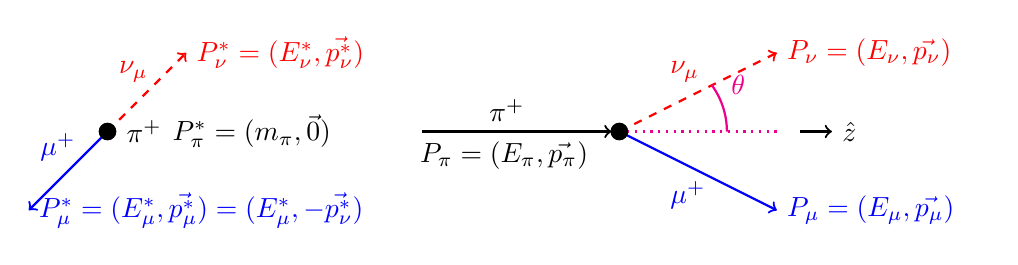
\begin{tikzpicture}
\draw[solid,thick,blue,->] (3,3) -- (2,2)
   node[above, midway, text width=2em]{$\mu^{+}$}
   node[right, text width=14em] {$P^{*}_{\mu}=(E_{\mu}^{*},\vec{p_{\mu}^{*}})=(E_{\mu}^{*},-\vec{p_{\nu}^{*}})$};
\draw[dashed,thick,red,->] (3,3) -- (4,4)
   node[above, midway, text width=2em]{$\nu_{\mu}$}
   node[right, text width=10em] {$P^{*}_{\nu}=(E_{\nu}^{*},\vec{p_{\nu}^{*}})$};
\filldraw (3,3) circle (3pt)
   node[right, text width=2em] {$\ \pi^{+}$}
   node[right, text width=10em] {$\ \ \ \ \ \ P^{*}_{\pi} = (m_{\pi},\vec{0})$};
\draw[solid,thick,black,->] (7,3) -- (9.4,3)
   node[above, midway, text width=2em] {$\pi^{+}$}
   node[below, midway, text width=7em] {$P_{\pi} = (E_{\pi},\vec{p_{\pi}})$};
\draw[dashed,thick,red, ->] (9.5,3) -- (11.5,4)
   node[above, midway, text width=2em] {$\nu_{\mu}$}
   node[right, text width=7em] {$P_{\nu} = (E_{\nu},\vec{p_{\nu}})$};
\draw[solid,thick,blue, ->] (9.5,3) -- (11.5,2)
   node[below, midway, text width=2em] {$\mu^{+}$}
   node[right, text width=7em] {$P_{\mu} = (E_{\mu},\vec{p_{\mu}})$};
\draw[dotted,thick,magenta ] (9.5,3) -- (11.5,3);
\filldraw (9.5,3) circle (3pt);
\draw [magenta,thick] ([shift=(30:1cm)]10,2.5) arc (0:36:1cm)
   node[right, text width=2em] {$\ \theta$};
\draw[solid,thick,black,->] (11.8,3) -- (12.2,3)
   node[right, text width=2em] {$\hat{z}$};
\end{tikzpicture}
}

\begin{columns}
  \begin{column}{0.44\textwidth}
    % Enu at CM
   \begin{block}{}
    {\color{red} \bf At the CM frame:}\\
    \vspace{0.3cm}
    {\small
     $P^{*}_{\pi} = P^{*}_{\mu} + P^{*}_{\nu}$\\
     $\Rightarrow P^{*}_{\pi} - P^{*}_{\nu} = P^{*}_{\mu}$\\
     $\Rightarrow (P^{*}_{\pi} - P^{*}_{\nu})^{2} = {P^{*}_{\mu}}^{2}$\\
     $\Rightarrow {P^{*}_{\pi}}^{2} + \cancel{{P^{*}_{\nu}}^{2}} - 2 \cdot P^{*}_{\pi} \cdot P^{*}_{\nu} = {P^{*}_{\mu}}^{2}$\\
     $\Rightarrow m_{\pi}^{2} - 2 \cdot m_{\pi} \cdot E_{\nu}^{*} = m_{\mu}^{2}$\\
     $\Rightarrow$ {\color{red} $E_{\nu}^{*} = (m_{\pi}^{2} - m_{\mu}^{2}) / (2 \cdot m_{\pi}) \ \ $} (1)\\
     $\Rightarrow$ {\color{red} \bf $E_{\nu}^{*} = 29.79 MeV$}
    }
   \end{block}
  \end{column}
  \begin{column}{0.02\textwidth}
  \end{column}
  \begin{column}{0.54\textwidth}
   {\color{red} \bf CM $\rightarrow$ LAB Lorentz transformation:}
   \begin{equation*}
     \begin{cases}
        {\color{magenta} E_{\nu} = \gamma \cdot (E_{\nu}^{*} + \beta \cdot (\vec{p_{\nu}^{*}}\cdot \hat{z}))} \ \ (2)\\
        \vspace{0.2cm}
        {\color{magenta} \vec{p_{\nu}}\cdot \hat{z} = \gamma \cdot (\beta \cdot E_{\nu}^{*} + \vec{p_{\nu}^{*}}\cdot \hat{z})} \ \ (3)
     \end{cases}
    \end{equation*}
    where:\\
      \vspace{0.1cm}
      \hspace{0.3cm} {\color{blue} $\vec{\beta} = \frac{\vec{p_{\pi}}}{E_{\pi}}$}  (4)\\
      \hspace{0.3cm} {\color{blue} $\gamma = (1-\vec{\beta}^{2})^{-1/2} = \frac{E_{\pi}}{m_{\pi}}$}  (5)\\
  \end{column}
\end{columns}

\end{frame}

%
%

\begin{frame}[t]{Going {\em off-axis}}

{\small
\begin{equation*}
   \vec{p_{\nu}}\cdot \hat{z} = p_{\nu} \cdot cos\theta
   \xRightarrow {p_{\nu} = E_{\nu}}
   \vec{p_{\nu}}\cdot \hat{z} = E_{\nu} \cdot cos\theta \ \ \ (6)
\end{equation*}

\vspace{0.1cm}
From Eq.\ (2) $\Rightarrow$
\begin{equation*}
  {\color{magenta} E_{\nu} - \gamma \cdot E_{\nu}^{*}} =
 {\color{blue} \underline{ \beta \cdot \gamma \cdot (\vec{p_{\nu}^{*}}\cdot \hat{z}) } } \ \ \ (7)
\end{equation*}

\vspace{0.1cm}
From Eqs.\ (3)(6) $\Rightarrow$
\begin{equation*}
  E_{\nu} \cdot cos\theta - \beta \cdot \gamma \cdot E_{\nu}^{*}  =  \gamma \cdot (\vec{p_{\nu}^{*}}\cdot \hat{z}) \Rightarrow
  {\color{magenta} \beta \cdot E_{\nu} \cdot cos\theta - {\beta}^{2} \cdot \gamma \cdot E_{\nu}^{*} } =
  {\color{blue} \underline{\beta \cdot \gamma \cdot (\vec{p_{\nu}^{*}}\cdot \hat{z})} }  \ \ \ (8)
\end{equation*}

\vspace{0.1cm}
From Eqs.\ (7)(8) $\Rightarrow$
\begin{equation*}
  E_{\nu} - \gamma \cdot E_{\nu}^{*} = \beta \cdot E_{\nu} \cdot cos\theta - {\beta}^{2} \cdot \gamma \cdot E_{\nu}^{*} \Rightarrow
  E_{\nu} \cdot (1 - \beta \cdot cos\theta) =  E_{\nu}^{*} \cdot \gamma \cdot (1 - {\beta}^{2}) = E_{\nu}^{*} / \gamma
\end{equation*}
\begin{equation*}
    \Rightarrow {\color{magenta} E_{\nu} = \frac{E_{\nu}^{*}}{\gamma \cdot (1 - \beta \cdot cos\theta)} } \ \ \ (9)
\end{equation*}
}
\noindent\rule{2cm}{0.4pt}\\
{\small
 Recall that
 {\color{magenta} $E_{\nu} = \gamma \cdot (E_{\nu}^{*} + \beta \cdot (\vec{p_{\nu}^{*}}\cdot \hat{z}))$} (2) and
 {\color{magenta} $\vec{p_{\nu}}\cdot \hat{z} = \gamma \cdot (\beta \cdot E_{\nu}^{*} + \vec{p_{\nu}^{*}}\cdot \hat{z})$} (3).
}

\end{frame}

%
%

\begin{frame}{Going {\em off-axis}}

\begin{flalign*}
   &E_{\nu}  = \frac {E_{\nu}^{*}} {\gamma \cdot (1 - \beta \cdot cos\theta)}
              \xRightarrow {cos\theta \approx 1 - {\theta}^{2}/2} & \\
   &E_{\nu}  = \frac {E_{\nu}^{*}} {\gamma \cdot (1 - \beta + \beta \cdot {\theta}^{2}/2)}
              \Rightarrow
    E_{\nu}  = \frac {E_{\nu}^{*}} {\gamma \cdot (1 - \beta) + \gamma \cdot \beta \cdot {\theta}^{2}/2)}
              \Rightarrow & \\
   &E_{\nu}  = \frac {E_{\nu}^{*} \cdot \gamma \cdot (1 + \beta)}
                    {{\gamma}^{2} \cdot (1 - \beta) \cdot (1 + \beta) + {\gamma}^{2} \cdot \beta \cdot (1+\beta) \cdot {\theta}^{2}/2)}
              \xRightarrow {(1 - \beta) \cdot (1 + \beta) = (1 - {\beta}^{2}) = 1/{\gamma}^{2}} & \\
   &E_{\nu}  = \frac {E_{\nu}^{*} \cdot \gamma \cdot (1 + \beta)}
                    {1 + {\gamma}^{2} \cdot \beta \cdot (1+\beta) \cdot {\theta}^{2}/2)}
              \xRightarrow {\beta \approx 1}
    E_{\nu}  = \frac {E_{\nu}^{*} \cdot 2\gamma}
                    {1 + {\gamma}^{2} \cdot {\theta}^{2}}
              \xRightarrow {Eq. (1)} & \\
   &E_{\nu}  = \frac{m_{\pi}^{2} - m_{\mu}^{2}} {\cancel{2} m_{\pi}} \cdot
               \frac {\cancel{2}\gamma} {1 + {\gamma}^{2} \cdot {\theta}^{2}}
              \xRightarrow{Eq. (3)}
    E_{\nu}  = \frac{m_{\pi}^{2} - m_{\mu}^{2}} {m_{\pi}} \cdot
               \frac {E_{\pi}/m_{\pi}} {1 + {(E_{\pi}/m_{\pi})}^{2} \cdot {\theta}^{2}}
              \Rightarrow & \\
   &E_{\nu}  = \frac{m_{\pi}^{2} - m_{\mu}^{2}} {{m_{\pi}}^{2}} \cdot
               \frac {E_{\pi}} {1 + {(E_{\pi}/m_{\pi})}^{2} \cdot {\theta}^{2}}
              \Rightarrow
   {\color{magenta}
    E_{\nu}  = (1 - \frac{m_{\mu}^{2}} {{m_{\pi}}^{2}}) \cdot
               \frac {{m_{\pi}}^{2} \cdot E_{\pi}} {{m_{\pi}}^{2} + {E_{\pi}}^{2} \cdot {\theta}^{2}}
   } \ \ (10) & \\
\end{flalign*}

\end{frame}

%
%

\begin{frame}{Going {\em off-axis}}

\begin{block}{}
\begin{equation*}
 {\color{magenta}
    E_{\nu}  = (1 - \frac{m_{\mu}^{2}} {{m_{\pi}}^{2}}) \cdot
               \frac {{m_{\pi}}^{2} \cdot E_{\pi}} {{m_{\pi}}^{2} + {E_{\pi}}^{2} \cdot {\theta}^{2}}
 }
\end{equation*}
\end{block}

\begin{columns}
  \begin{column}{0.50\textwidth}
    \begin{itemize}
      \item {\color{red} \bf $\theta = 0$} (on-axis beam): \\
        \begin{itemize}
          \item $\displaystyle E_{\nu}  = (1 - \frac{m_{\mu}^{2}} {{m_{\pi}}^{2}}) \cdot  E_{\pi}$
          \item Neutrino energy proportional to the pion energy
        \end{itemize}
      \item {\color{red} \bf $E_{\pi} \cdot \theta >> m_{\pi}$}: \\
        \begin{itemize}
          \item $\displaystyle E_{\nu}  = (1 - \frac{m_{\mu}^{2}} {{m_{\pi}}^{2}}) \cdot \frac {{m_{\pi}}^{2}} {E_{\pi} \cdot {\theta}^{2}}$
          \item Higher energy pions contribute to the low energy neutrino flux
        \end{itemize}
    \end{itemize}
  \end{column}
  \begin{column}{0.50\textwidth}
     \includegraphics[width=0.95\textwidth]{./images/3nu/accelerator/offaxis_angle_epi_vs_enu_degrees.png}
  \end{column}
\end{columns}

\end{frame}

} % done with off-axis beam details



%
%
\begin{frame}{Near detector complex}

  \begin{center}
    \includegraphics[width=0.90\textwidth]{./images/3nu/accelerator/t2k/nd_complex_2}
  \end{center}

\end{frame}


%
% Beam monitoring - nu
%
\begin{frame}{T2K neutrino beam monitoring}
\begin{columns}
  \begin{column}{0.35\textwidth}
     \includegraphics[width=0.99\textwidth]{./images/3nu/accelerator/t2k/INGRID_picture_1.jpg}
  \end{column}
  \begin{column}{0.65\textwidth}
     \includegraphics[width=0.45\textwidth]{./images/3nu/accelerator/t2k/INGRID_schematic_3.png}
     \includegraphics[width=0.45\textwidth]{./images/3nu/accelerator/t2k/INGRID_event_display_1.png}
     \begin{itemize}
       {\small
        \item 16 modules (14 in cross configuration).
        \item Each module: 7 tons, alternating scintillator / iron planes.
        \item 10 m $\times$ 10 m beam area coverage
        \item 1 event per $\sim$6$\times$10$^{13}$ protons on target.
        \item Monitors neutrino beam rate and profile.
        }
     \end{itemize}
  \end{column}
\end{columns}
\end{frame}


%
%
\begin{frame}{T2K neutrino beam monitoring}

\begin{columns}
  \begin{column}{0.65\textwidth}
   \begin{center}
    \includegraphics[width=0.90\textwidth]{./images/3nu/accelerator/t2k/beam_monitoring}\\
   \end{center}
  \end{column}
  \begin{column}{0.35\textwidth}
    \begin{itemize}
      {\small
      \item Beam direction stable within 1 mrad (corresponding to less than $\sim$2\% peak energy shift at SuperK)
      \item POT (Protons On Target) normalised event rate stable to better than 1\%
      }
    \end{itemize}
  \end{column}
\end{columns}
\end{frame}

%
%
%
\begin{frame}{T2K off-axis Near Detector at 280 m}

  \begin{center}
   \includegraphics[width=0.85\textwidth]{./images/3nu/accelerator/t2k/nd280_photo.png}
  \end{center}

\end{frame}

%
%
%
\begin{frame}{T2K off-axis Near Detector at 280 m}

{\small
Tracking Calorimeters and Time Projection Chambers in a 0.2 T B field.\\
Polystyrene and water targets.}

\begin{center}
  \includegraphics[width=0.80\textwidth]{./images/3nu/accelerator/t2k/nd280_schematic.png}
\end{center}

\end{frame}

%
%
%
\begin{frame}{Tracker system @ T2K off-axis Near Detector at 280 m}

  \begin{center}
   \includegraphics[width=0.70\textwidth]{./images/3nu/accelerator/t2k/nd280_tracker_event.png}
  \end{center}

  \begin{itemize}
   {\scriptsize
   \item 2 fine-grained scintillator detectors (FGDs) + 3 time projection chambers (TPCs).
   \item FGDs provide the target mass\\ (FGD1: 1 ton scintillator, FGD2: 0.5 ton scintillator + 0.5 ton water).
   \item Momentum measurement of charged particles, PID via dE/dx.
   \item Better than 10\% dE/dx resolution, and 10\% momentum resolution at 1 GeV.\\
   }
  \end{itemize}

\end{frame}

%
%
%
\begin{frame}{The T2K Far Detector (Super-Kamiokande IV)}
\begin{columns}
  \begin{column}{0.45\textwidth}
     \includegraphics[height=0.85\textheight]{./images/3nu/accelerator/t2k/superk_inside_view_portrait_1.jpg}
  \end{column}
  \begin{column}{0.55\textwidth}
  {\small
  \begin{itemize}
    \item 50 kt Water Cherenkov detector\\ (22.5 kton fiducial)
    \item Overburden (shielding): 2700 mwe
    \item Inner Detector (ID): 11,129 20'' PMTs\\ (40\% photo-cathode coverage)
    \item Outer Detector (OD): 1,885 8'' PMTs
    \item DAQ: No dead-time
    \item Energy threshold: $\sim$ 4.5 MeV
  \end{itemize}
  }
  \end{column}
\end{columns}
\end{frame}

%
%
%
\begin{frame}{Water Cherenkov Imaging}

  \begin{center}
   \includegraphics[width=0.85\textwidth]{./images/3nu/accelerator/t2k/superk_3d_event_display}
  \end{center}

\end{frame}

%
%
%
\begin{frame}{Water Cherenkov Imaging: Identifying $\pbar{\nu}_{e}$ and  $\pbar{\nu}_{\mu}$}

\begin{center}
  \includegraphics[width=0.90\textwidth]{./images/3nu/accelerator/t2k/event_displays_1mu_1e_bkg}
\end{center}

\end{frame}

%
%
%
\begin{frame}{Water Cherenkov Imaging: Identifying $\pbar{\nu}_{e}$ and  $\pbar{\nu}_{\mu}$}

  \begin{itemize}
    \item Excellent e/$\mu$ separation.
    \item Probability to misidentify a muon as an electron is smaller than 1\%.
  \end{itemize}

  \begin{center}
   \includegraphics[width=0.85\textwidth]{./images/3nu/accelerator/t2k/emuPID}
  \end{center}

\end{frame}

%
%
%

\begin{frame}{The NOvA experiment (2013-present)}

\begin{columns}
  \begin{column}{0.45\textwidth}
     \includegraphics[width=0.99\textwidth]{./images/3nu/accelerator/nova_fnal}
  \end{column}
  \begin{column}{0.55\textwidth}
  \begin{itemize}
  {\scriptsize
    \item Relatively pure $\nu_{\mu}$ ($\bar{\nu}_{\mu}$) beam.
    \item Produced using the 120-GeV Main Injector proton beam at FNAL (same as MINOS)
    \item Achieved $>$ 700 kW (working towards $>$ 700 kW)
    \item Functionally identical near and far detectorss: Extruded PVC with mineral oil as scintillator,
    and avalance photodiodes for light collection.
    \item Both detectors 0.8 degrees (14 mrad) off-axis.
    \item Near detector at FNAL (1 km from target): 300 tonnes
    \item Far detector at Ash River (810 km from target): 14,000 tonnes
    \item Neutrino flux at Ash River peaked at $\sim$2.0 GeV.
    \item L/E tuned to the `atmospheric' ${\Delta}m^{2}$ ($\sim$2.4$\times$10$^{-3}$ $eV^{2}/c^{4}$).
  }
  \end{itemize}
  \end{column}
\end{columns}
\end{frame}

%
%
%

\begin{frame}{The NOvA flux}

  \begin{columns}
    \begin{column}{0.55\textwidth}
       \includegraphics[width=0.99\textwidth]{./images/3nu/accelerator/nova_flux}
    \end{column}
    \begin{column}{0.45\textwidth}
      \begin{itemize}
      {\scriptsize
        \item Relatively pure $\nu_{\mu}$ ($\bar{nu}_{\mu}$) beam.
        \item Produced using the 120-GeV Main Injector proton beam at FNAL (same as MINOS)
        \item Achieved $>$ 700 kW (working towards $>$ 700 kW)
        \item Both detectors 0.8 degrees (14 mrad) off-axis.
        \item Neutrino flux at Ash River peaked at $\sim$2.0 GeV.
      }
      \end{itemize}
    \end{column}
  \end{columns}

\end{frame}
%
%
%

\begin{frame}{The NOvA detectors}

  \begin{center}
   \includegraphics[width=0.85\textwidth]{./images/3nu/accelerator/nova_detectors}
  \end{center}

\end{frame}

%
%
%

\begin{frame}{Event signatures in NOvA}
\begin{center}
  \includegraphics[width=0.65\textwidth]{./images/3nu/accelerator/nova_events}
\end{center}
\end{frame}


%
%
%

\begin{frame}{First experimental hints by T2K and MINOS}

  \underline{2011 T2K result} - About a year after the start of T2K physics data taking.\\
  6 events with a background of 1.5 $\pm$ 0.3 (syst) events:
  {\bf A 2.5$\sigma$ excess}. \\

  \begin{columns}
    \begin{column}{0.60\textwidth}
      \begin{center}
       \includegraphics[width=0.75\textwidth]{./images/3nu/accelerator/t2knueapp_first}\\
       \vspace{0.3cm}
       {\scriptsize \color{blue}[Phys.Rev.Lett. 107 (2011) 041801}
      \end{center}
    \end{column}
    \begin{column}{0.40\textwidth}
         \vspace{0.3cm}
         \begin{center}
         At about the same time, with nearly final exposure,
         MINOS was reporting a {\bf 1.7$\sigma$ excess.}\\
         \includegraphics[width=0.95\textwidth]{./images/3nu/accelerator/minos_nueapp}\\
         \vspace{0.3cm}
         NOvA was not online yet.
         \end{center}
    \end{column}
  \end{columns}

\end{frame}


\begin{frame}{}

  \begin{center}
   Convincing early evidence for $\theta_{13} \ne 0$: Needed more data for discovery.\\
   \vspace{0.2cm}
   \includegraphics[width=0.95\textwidth]{./images/3nu/accelerator/tohoku_earthquake}\\
  \end{center}

\end{frame}

%
%
%

\begin{frame}{SBL reactor experiments coming online (ca 2011)}

\begin{itemize}
  \item {\bf Daya Bay}, South China (6: 12/2011-07/2012, 8: 10/2012-12/2016)
     \begin{itemize}
        \item Reactors: 6 cores, 17.6 $GW_{th}$ total
        \item Far detector: 4 functionally identical far detectors $\times$ 20 tonnes target mass each
                 (80 tonnes total mass),
                 1615 - 1985 m from cores
                 %350 m overburden
        \item Near detector: 4 functionally identical near detectors $\times$ 20 tonnes target mass each,
                 363-526 m from cores
                 %$\sim$ 100 m overburden
     \end{itemize}
  \item {\bf RENO}, South Korea %(08/2011-)
     \begin{itemize}
       \item Reactors: 6 cores, 16.4 $GW_{th}$ total
       \item Far detector: 16.5 tonnes target mass, 290 m from cores
       \item Near detector: 16.5 tonnes target mass, 1380 m from cores
     \end{itemize}
  \item Double CHOOZ, France
     \begin{itemize}
        \item Reactors: 2 cores, 8.7 $GW_{th}$ total
        \item Far detector: 8.2 tonnes target mass, 1067 m from cores
              %, 300 mwe overburden
        \item Near detector: 8.2 tonnes target mass, 410 m from cores
              %, 115 mwe overburden
     \end{itemize}
\end{itemize}

\end{frame}


\begin{frame}{The Daya Bay experiment (others similar)}

\centering
\includegraphics[width=0.80\textwidth]{./images/3nu/reactor/dayabay_configuration.png}\\
{\scriptsize \color{blue}[Chao Zang, Neutrino 2014, Boston]}
\end{frame}


\begin{frame}{The Daya Bay experiment (others similar)}

\begin{columns}
  \begin{column}{0.33\textwidth}
   \centering
     \includegraphics[width=0.99\textwidth]{./images/3nu/reactor/dayabay_1AD.png}\\
     \includegraphics[width=0.80\textwidth]{./images/3nu/reactor/dayabay_photo.png}\\
  \end{column}
  \begin{column}{0.66\textwidth}
    \begin{itemize}
    {\small
      \item Three cylindrical zone design:\\
        \begin{itemize}
        {\small
          \item {\bf Inner}: 20 tonnes of Gd-doped (0.1\% in weight) liquid scintillator
          \item {\bf Middle}: 22 tonnes of liquid scintillator
          \item {\bf Outer}: 40 tonnes of mineral oil
        }
        \end{itemize}
      \item 192 8'' photosensors installed in each detector (8\% photo-cathode coverage)
      \item Each detector placed within high purity water to further reduce background
      \item Water pools divided in optically separated regions (inner and outer) and instrumented with photo-sensors.
      \item Backgrounds: accidental, fast neutrons, $^{9}$Li and $^{8}$He spallation products,
            internal radioactivity and correlated background from Am-C calibration source
    }
    \end{itemize}
  \end{column}
\end{columns}
\end{frame}


%
%
%

\begin{frame}{Early SBL reactor experiment results}

Once the reactor experiments switched on, the the hunt for $\theta_{13}$ was over.

\begin{itemize}
  \item Daya Bay produced 5.2$\sigma$ evidence of non-zero $\theta_{13}$
        after less than 2 months of data-taking
        {\scriptsize \color{blue} [Phys.Rev.Lett. 108 (2012) 171803]}
  \item RENO followed just 2 weeks later with
        4.9$\sigma$ evidence of non-zero $\theta_{13}$ (222 days)
\end{itemize}

\end{frame}

%
%
%

\begin{frame}{Early SBL reactor experiment results}

\begin{columns}
  \begin{column}{0.60\textwidth}
    \centering
     \includegraphics[width=0.85\textwidth]{./images/3nu/reactor/dayabay_results_spectrum_2014.png}\\
     {\scriptsize \color{blue}[plots from Chao Zang, Seon-Hee Seo and De Kerret, Neutrino 2014, Boston]}
  \end{column}
  \begin{column}{0.40\textwidth}
    \centering
     \includegraphics[width=0.99\textwidth]{./images/3nu/reactor/reno_results_spectrum_2014.png}\\
     \includegraphics[width=0.99\textwidth]{./images/3nu/reactor/doublechooz_results_spectrum_2014.png}
  \end{column}
\end{columns}
\end{frame}

%
%
%

\begin{frame}{Final Daya Bay results}

Data from 1958 days of data collection, with nearly 4M $\bar{\nu}_e$ IBD events.

\vspace{0.1cm}

\begin{columns}
  \begin{column}{0.50\textwidth}
    \centering
     \includegraphics[width=0.90\textwidth]{./images/3nu/reactor/daya_bay_final_2018_spectrum}\\
  \end{column}
  \begin{column}{0.50\textwidth}
    \centering
     \includegraphics[width=0.90\textwidth]{./images/3nu/reactor/daya_bay_final_2018_osc_params}\\
  \end{column}
\end{columns}

\vspace{0.1cm}

{\scriptsize \color{blue}[Daya Bay Collaboration, Phys.Rev.Lett. 121 (2018) 241805}

\noindent\rule{2cm}{0.4pt}\\
{\scriptsize
  $\Delta m^2_{ee}$ is defined as
  $\Delta m^2_{32} +
  \frac{2E}{L} arctan\Big(\frac{sin2\Delta_{21}}{cos2\Delta_{21}+tan^{2}\theta_{12}}\Big)$
  where $\Delta_{ij}=\Delta m^2_{ij}L/(4E)$.\\
  For a discussion, see {\color{blue} [J.Parke et al., arXiv:1903.00148]}
}

\end{frame}

%
%
%

% \begin{frame}{Updated RENO results}
%
%
% \end{frame}


%
%
%

\begin{frame}{$\nu_e$ appearance observation (T2K)}

  Finishing the job once data taking resumed:\\
  \vspace{0.2cm}
  \begin{center}
   \includegraphics[width=0.99\textwidth]{./images/3nu/accelerator/t2k_nueapp_obs}\\
  \end{center}

\end{frame}

%
%
%

\begin{frame}{(Almost) $\bar{\nu}_e$ appearance observation (NOvA)}

  \begin{columns}[T]
    \begin{column}{0.40\textwidth}
       \includegraphics[width=0.90\textwidth]{./images/3nu/accelerator/nova_nuebar_app2019.png}
    \end{column}
    \begin{column}{0.60\textwidth}
       NOvA (left):
       \begin{itemize}
         \item 27 $\nu_e$ CC-like candidates
         \item Estimated background: 10.3$^{+0.6}_{-0.5}$ events
         \item {\bf 4.4$\sigma$ excess}
       \end{itemize}
       \vspace{0.2cm}
       [{\color{blue} \scriptsize NOvA Collaboration, PRL 123 (2019) no.15, 151803}]\\
       \vspace{0.5cm}
       T2K:
       \begin{itemize}
         \item 15 $\nu_e$ CC-like candidates
         \item Estimated background: 9.3 events
       \end{itemize}
       \vspace{0.2cm}
       [{\color{blue} \scriptsize T2K Collaboration, PRL 124 (2020) no. 16, 161802}]\\

    \end{column}
  \end{columns}

\end{frame}

%
%
%

\begin{frame}{Precision $\nu_{\mu}(\bar{\nu}_{\mu})$ disap. measurements by T2K/NOvA}

\begin{center}
  \includegraphics[width=0.65\textwidth]{./images/3nu/accelerator/nova_disapp_2020}
  \includegraphics[width=0.65\textwidth]{./images/3nu/accelerator/t2k_disapp_2020_2}
\end{center}

\end{frame}

\begin{frame}{Precision $\nu_{\mu}(\bar{\nu}_{\mu})$ disap. measurements by T2K/NOvA}

\begin{center}
  \includegraphics[width=0.90\textwidth]{./images/3nu/accelerator/acc_lbl_disapp_limits}
\end{center}

\end{frame}

%
%
%

\begin{frame}{Global picture: $\theta_{13}$ and $|\Delta m^{2}_{32}|$}

\begin{center}
\includegraphics[width=0.98\textwidth]{./images/3nu/reactor/global_theta13_and_dmsq32}
\end{center}

\end{frame}

%
%
%

%
% --------------------------------------------------
%
% Measuring CP - The main idea
%
% --------------------------------------------------
%
\begin{frame}{}

\begin{center}
Precise measurement of $\theta_{13}$ by SBL reactor experiments.\\
\vspace{0.2cm}
Strong $\pbar{\nu}_{\mu} \rightarrow \pbar{\nu}_{e}$ signals in LBL accelerator experiments.\\
\vspace{0.5cm}
{\bf An opportunity was presented for LBL accelerator experiments to measure leptonic CPV!}
\vspace{1.5cm}
\includegraphics[width=0.98\textwidth]{./images/osc101/numu2nue_full}
\end{center}

\end{frame}

%
%
%
\begin{frame}{Leptonic CP violation?}

The CP-violating phase in PMNS is largely unconstrained.\\
\vspace{0.2cm}
The magnitude of the CP effect  is given by the {\bf Jarlskog Invariant}:
\begin{equation*}
  J_{CP}^{{\color{amber}PMNS}} = \frac{1}{8} \; sin2\theta_{12} \; sin2\theta_{13} \;
     sin2\theta_{23} \; cos\theta_{13} \; {\color{magenta}
       sin\delta_{CP} }
\end{equation*}

Given the current best fit values, and assuming the normal hierarchy:
\begin{equation*}
  J_{CP}^{{\color{amber}PMNS}} = 0.035 \; {\color{magenta}sin\delta_{CP}}
\end{equation*}

In contrast, in the quark sector, despite the large value of the
CP phase:
\begin{equation*}
  J_{CP}^{{\color{capri}CKM}} \approx  (3 \pm 1) \times 10^{-5}
\end{equation*}

$J_{CP}^{{\color{amber}PMNS}}$ is {\bf potentially large!} \\
\vspace{0.2cm}
Measurement of leptonic CPV could have a tremendous impact on our understanding of the
origin of the {\bf Baryon Asymmetry of the Universe}.

\end{frame}

%
%
\begin{frame}{Measuring $\delta_{CP}$}

\begin{columns}
  \begin{column}{0.60\textwidth}
    \begin{center}
      \includegraphics[width=0.99\textwidth]{./images/biprob/biprob_expt_hiprecision}
    \end{center}
  \end{column}
  \begin{column}{0.40\textwidth}
  {\small
       If CP is violated:
       \begin{equation*}
       {\color{magenta}
          P(\nu_{\mu} \rightarrow \nu_{e}) \ne
          P(\bar{\nu}_{\mu} \rightarrow \bar{\nu}_{e})
       }
       \end{equation*}
       \vspace{0.2cm}
       So a measurement in the
       \begin{equation*}
          \Big(
            {\color{magenta}
                 P(\nu_{\mu} \rightarrow \nu_{e}) }
           ,
            {\color{magenta}
                 P(\bar{\nu}_{\mu} \rightarrow \bar{\nu}_{e}) }
          \Big)
       \end{equation*}
       space will be off the diagonal.\\
      \vspace{0.4cm}
       Within the standard 3-flavour model, the only source of CP
       violation is the $\delta_{CP}$ phase:\\ This measurement can
       be used to determine the value of  $\delta_{CP}$.
  }
  \end{column}
\end{columns}

\end{frame}

%
%
\begin{frame}{Measuring $\delta_{CP}$}

{\small
       Within the standard 3-flavour model, the only source of CP
       violation is the $\delta_{CP}$ phase:
       It enters as an
       $e^{{\pm}i\delta_{CP}}$ term, so it has a {\bf cyclical effect}.
}

\begin{columns}
  \begin{column}{0.60\textwidth}
    \begin{center}
       \includegraphics[width=0.99\textwidth]{./images/biprob/biprob_expt_hiprecision_good_ellipse_vac_maximal}
    \end{center}
  \end{column}
  \begin{column}{0.40\textwidth}
  {\small
       Note that:
      \begin{itemize}
      {\scriptsize
         \item Points for $\delta_{CP}$ = 0 or $\pi$ are on the diagonal (no CP).
         \item $\pi$/2 corresponds to more $\bar{\nu}_e$ appearance
         \item 3$\pi$/2 (-$\pi$/2) corresponds to more $\nu_e$
           appearance
      }
      \end{itemize}
  }
  \end{column}
\end{columns}

\end{frame}


%
%
\begin{frame}{Measuring $\delta_{CP}$}

{\small
      Unfortunatelly, T2K is less able to disciminate between the
      CP conserving values of $\delta_{CP}$ (0, $\pi$), so the ellipse
      is flattened.
}

\begin{columns}
  \begin{column}{0.60\textwidth}
    \begin{center}
       \includegraphics[width=0.99\textwidth]{./images/biprob/biprob_t2k_vac_maximal}
    \end{center}
  \end{column}
  \begin{column}{0.40\textwidth}
  {\small
      Large ranges of $\delta_{CP}$ values give nearly-identical
      asymmetry:\\ Difficult to do much more than just discriminating
      between the\\ (0, $\pi$) and ($\pi$, 2$\pi$) ranges...\\
      \vspace{0.2cm}
      So the T2K $\delta_{CP}$ measurement resolution is quite poor.\\
      \vspace{0.2cm}
      This is made even worst by matter effects, ignored in this plot
      (vacuum oscillation probabilities are shown).\\
   }
  \end{column}
\end{columns}

\end{frame}

%
%
\begin{frame}{Measuring $\delta_{CP}$}

Matter effect can play an important role in neutrino oscillations.

\begin{equation*}
   A_{CP} = \frac
     {P(\nu_{\mu} \rightarrow \nu_{e}) - P(\bar{\nu}_{\mu} \rightarrow \bar{\nu}_{e})}
     {P(\nu_{\mu} \rightarrow \nu_{e}) + P(\bar{\nu}_{\mu} \rightarrow \bar{\nu}_{e})}
\end{equation*}

In the 3-flavour model, $A_{CP}$ can be approximated as:
\begin{equation*}
   A_{CP} \approx \frac
    {cos\theta_{23} sin2\theta_{12} {\color{magenta} sin\delta_{CP}}}
    {sin\theta_{23} sin\theta_{13}}
    \Big( \frac{{\Delta}m^2_{21}L}{4E} \Big) +
    {\color{magenta} \; matter \; effects}
\end{equation*}

Matter induced asymmetry in
$P(\nu_{\mu} \rightarrow \nu_{e})$,
$P(\bar{\nu}_{\mu} \rightarrow \bar{\nu}_{e})$
in addition to CP.\\

% In general:
% \begin{equation*}
%    A_{CP} \propto L / E \;\;\;\; and \;\;\;\;
%    A_{matter} \propto L \cdot E
% \end{equation*}

\vspace{0.4cm}

Experimental sensitivity to CP violation and the MH from measurements
of the total asymmetry between
$P(\nu_{\mu} \rightarrow \nu_{e})$,
$P(\bar{\nu}_{\mu} \rightarrow \bar{\nu}_{e})$
requires the {\bf disambiguation of the asymmetries} induced by matter and CP
violation.

\end{frame}


%
%
\begin{frame}{Measuring $\delta_{CP}$}

{\small
 Matter effect can play an important role in neutrino oscillations.
}

\begin{columns}
  \begin{column}{0.60\textwidth}
    \begin{center}
       \includegraphics[width=0.99\textwidth]{./images/biprob/biprob_t2k_matter_maximal}
    \end{center}
  \end{column}
  \begin{column}{0.40\textwidth}
  {\small
      Important to know the MH.
      \begin{itemize}
      {\small
         \item For NH, $\nu_e$ appearance is enhanced and
           $\bar{\nu}_e$ appearance is suppressed.
         \item For IH, $\nu_e$ appearance is suppressed and
           $\bar{\nu}_e$ appearance is enhanced.
      }
      \end{itemize}
      \vspace{0.1cm}
      Matter effects useful for lifting degeneracies,
      identifying the hierarchy and measuring $\delta_{CP}$.\\
      \vspace{0.1cm}
      T2K: Not enough matter effect!
  }
  \end{column}
\end{columns}

\end{frame}

%
%
\begin{frame}{Measuring $\delta_{CP}$}

\begin{columns}[T]
  \begin{column}{0.50\textwidth}
    \begin{center}
       {\bf Example: NOvA}\\
       \includegraphics[width=0.99\textwidth]{./images/biprob/biprob_nova_matter_maximal}
    \end{center}
  \end{column}
  \begin{column}{0.50\textwidth}
    \begin{center}
       {\bf Example: DUNE}\\
       \includegraphics[width=0.99\textwidth]{./images/biprob/biprob_dune_matter_maximal}
    \end{center}
  {\small
  }
  \end{column}
\end{columns}

\end{frame}

%
%
\begin{frame}{Measuring $\delta_{CP}$}

The $\theta_{23}$ {\bf octant degeneracy} further limits our CP sensitivity
and measurement resolution.

\begin{columns}
  \begin{column}{0.65\textwidth}
    \begin{center}
       \includegraphics[width=0.99\textwidth]{./images/biprob/biprob_t2k_matter_non_maximal}
    \end{center}
  \end{column}
  \begin{column}{0.35\textwidth}
  {\small
   \begin{center}
       $1 - P(\nu_{\mu}\rightarrow\nu_{\mu}) \propto sin^{2}{\color{magenta}2}\theta_{23}$
   \end{center}
   \vspace{0.2cm}
   \begin{center}
       $P(\nu_{\mu}\rightarrow\nu_{e}) \propto sin^{2}\theta_{23}$
   \end{center}
  }
  \end{column}
\end{columns}

\end{frame}

%
%
\begin{frame}{Measuring $\delta_{CP}$}

T2K could exclude the  `{\color{magenta}$sin\delta_{CP}$=0, $\pi$}'
(conserved CP) hypothesis, at some modest
significance level, and only if the true $\delta_{CP}$ value lies in a
very favourable region...

\begin{columns}[T]
  \begin{column}{0.50\textwidth}
    \begin{center}
       \includegraphics[width=0.99\textwidth]{./images/biprob/biprob_expt_poorprecision_t2k_matter_non_maximal}
    \end{center}
  \end{column}
  \begin{column}{0.50\textwidth}
    \begin{center}
      {\small
         True MH: NH, Full T2K exposure,\\ 50\% $\nu$ - 50\% $\bar{\nu}$\\
       }
       \includegraphics[width=0.99\textwidth]{./images/biprob/exclude_sindelta0_50nu50nubar_nh_selected_theta23}
    \end{center}
  \end{column}
\end{columns}

\end{frame}


%
%
%

% \begin{frame}{T2K $\nu_{\mu}$ event spectra}
%
%   \begin{center}
%      \includegraphics[width=0.99\textwidth]{./images/3nu/accelerator/t2k_wasco_nu2018_1}
%   \end{center}
%
% \end{frame}
%
% \begin{frame}{T2K $\nu_{\mu}$ disappearance}
%
%   \begin{center}
%      \includegraphics[width=0.99\textwidth]{./images/3nu/accelerator/t2k_wasco_nu2018_2}
%   \end{center}
%
% \end{frame}
%
% \begin{frame}{T2K $\nu_{\mu}$ appearance}
%
%   \begin{center}
%      \includegraphics[width=0.99\textwidth]{./images/3nu/accelerator/t2k_wasco_nu2018_3}
%   \end{center}
%
% \end{frame}
%
% \begin{frame}{T2K $\nu_{\mu}$ CPV}
%
%   \begin{center}
%      \includegraphics[width=0.99\textwidth]{./images/3nu/accelerator/t2k_wasco_nu2018_4}
%   \end{center}
%
% \end{frame}

%
%
%

\begin{frame}{CPV at T2K}

  \begin{columns}[T]
    \begin{column}{0.40\textwidth}
      \begin{center}
         \includegraphics[width=0.95\textwidth]{./images/3nu/accelerator/t2k_cpv_nature2019_spectra}\\
      \end{center}
    \end{column}
    \begin{column}{0.60\textwidth}
      \begin{center}
         \includegraphics[width=0.90\textwidth]{./images/3nu/accelerator/t2k_cpv_nature2019_nevent_table}\\
      \end{center}
      \vspace{0.3cm}
      [{\color{blue} \scriptsize T2K Collaboration, Nature 580 (2020) 7803, 339-344}]\\
    \end{column}
  \end{columns}

\end{frame}

%
%
%

\begin{frame}[t]{CPV at T2K}

  \begin{columns}[T]
    \begin{column}{0.40\textwidth}
      \begin{center}
         \includegraphics[width=0.99\textwidth]{./images/3nu/accelerator/t2k_cpv_2019}\\
      \end{center}
    \end{column}
    \begin{column}{0.60\textwidth}
      \begin{itemize}
        {\small
        \item Confidence intervals at the 68.27\% CL for $\delta_{CP}$ vs $sin^{2}\theta_{13}$ (NO)
        \item Confidence intervals at the 68.27\% and 99.73\% CL for $\delta_{CP}$ vs $sin^{2}\theta_{23}$ (NO)
        \item Confidence intervals  68.27\% and 99.73\% CL on $\delta_{CP}$
        \begin{itemize}
          {\small
          \item Credible interval marginalised across both mass orderings excludes 42\% of the
                available space at 3$\sigma$.
          \item CP conserving values strongly disfavoured.
          }
        \end{itemize}
        }
      \end{itemize}
      [{\color{blue} \scriptsize T2K Collaboration, Nature 580 (2020) 7803, 339-344}]\\
    \end{column}
  \end{columns}

\end{frame}

%
%
%

\begin{frame}{CPV at NOvA}

  \begin{columns}[T]
    \begin{column}{0.45\textwidth}
      \begin{center}
         \includegraphics[width=0.95\textwidth]{./images/3nu/accelerator/nova_cpv_2020}\\
      \end{center}
    \end{column}
    \begin{column}{0.55\textwidth}
      \begin{itemize}
        {\small
        \item Confidence intervals at the 1$\sigma$, 2$\sigma$, and 3$\sigma$
              for $\delta_{CP}$ vs $sin^{2}\theta_{23}$ (NO, IO)
        \begin{itemize}
          {\small
          \item IO disfavoured at $\sim$2$\sigma$
          \item CP conserving values allowed even within 1$\sigma$
          }
        \end{itemize}
        }
      \end{itemize}
      [{\color{blue} \scriptsize NOvA Collaboration, Neutrino 2020}]\\

      \begin{center}
         \includegraphics[width=0.99\textwidth]{./images/3nu/accelerator/t2k_nova_tensions}\\
      \end{center}

    \end{column}
  \end{columns}

\end{frame}

%
%
%

\begin{frame}{A new anomaly brewing?}

  \begin{columns}[T]
    \begin{column}{0.40\textwidth}
      \begin{center}
         \includegraphics[width=0.80\textwidth]{./images/3nu/accelerator/nova_biprob_data}\\
      \end{center}
    \end{column}
    \begin{column}{0.60\textwidth}
      \begin{center}
         \includegraphics[width=0.99\textwidth]{./images/3nu/accelerator/t2k_biprob_data}\\
      \end{center}
    \end{column}
  \end{columns}

\end{frame}

%
%
%

% \begin{frame}{What to read}
%
% {\color{magenta} Add in next revision}
%
% \end{frame}


% \begin{frame}{T2K $\nu_{\mu}$ disappearance}
%
% {\small
% 446.0 $\pm$ 22.5 (syst.) single-ring $\mu$-like events expected in absence of oscillations
% but only 120 events were observed
% (Run 1-4: 6.57$\times$10$^{20}$ POT, $\sim$ first 10\% of the final exposure).
% The observed deficit is strongly energy-dependent.
% }
% \begin{columns}[T]
%   \begin{column}{0.50\textwidth}
%      \includegraphics[width=0.98\textwidth]{./images/3nu/accelerator/t2k/run1to4_disapp_spectrum.png}\\
%   \end{column}
%   \begin{column}{0.50\textwidth}
%      \includegraphics[width=0.99\textwidth]{./images/3nu/accelerator/t2k/run1to4_disapp_contour.png}\\
%   \end{column}
% \end{columns}
% \begin{itemize}
% {\small
%       \item
%        The dramatic energy dependent deficit allows T2K to place
%        very stringent constraints on $\nu_{\mu}$ disappearance parameters.
%       \item
%        NH:
%         $|\Delta m^{2}_{32}|$ = (2.51 $\pm$ 0.10) $\times10^{-3} eV^{2}/c^{4}$ and
%         $\sin^{2}\theta_{23}$ = 0.514 $^{+0.055}_{-0.056}$
%       \item
%        Some tension with the MINOS results.
% }
% \end{itemize}
% \end{frame}
%
%
% %
% %
% %
% \begin{frame}{T2K $\nu_{e}$ appearance}
%
% {\small
%  28 1-ring e-like events were observed, with an expected background of 4.92 $\pm$ 0.55 (syst) events.
%  The significance of the excess is 7.3$\sigma$ (first ever observation of an explicit appearance signal).\\
% }
%
% \vspace{0.5cm}
%
% \begin{columns}
%   \begin{column}{0.60\textwidth}
%      \includegraphics[width=0.99\textwidth]{./images/3nu/accelerator/t2k/ptheta_with_proj_nh.png}
%   \end{column}
%   \begin{column}{0.40\textwidth}
%      \includegraphics[width=0.99\textwidth]{./images/3nu/accelerator/t2k/nexp_st13_categories.png}\\
% %     \includegraphics[width=0.99\textwidth]{./images/3nu/accelerator/t2k/nexp_error_summary_table.png}\\
%      \vspace{0.2cm}
%      {\scriptsize
%       Best fit value of $\sin^{2}2\theta_{13}$ \\ (for $\delta_{CP}=0$, $|\Delta m^{2}_{32}|$ = 2.4$\times10^{-3} eV^{2}/c^{4}$
%       and $\sin^{2}\theta_{23}$ = 0.5):
%       \begin{itemize}
%          \item $\sin^{2}2\theta_{13}$ = 0.14 (Normal)
%          \item $\sin^{2}2\theta_{13}$ = 0.17 (Inverted)
%       \end{itemize}
%       }
%   \end{column}
% \end{columns}
% \end{frame}
%
%
% %
% %
% %
% \begin{frame}{T2K constraint on $\theta_{13}$}
% \begin{columns}
%   \begin{column}{0.50\textwidth}
%
%      \includegraphics[width=0.90\textwidth,height=0.42\textheight]{./images/3nu/accelerator/t2k/real_result_lh21_rn22_mh0_st2340_dl.png}\\
%      \includegraphics[width=0.90\textwidth,height=0.42\textheight]{./images/3nu/accelerator/t2k/real_result_lh21_rn22_mh1_st2340_dl.png}\\
%   \end{column}
%   \begin{column}{0.50\textwidth}
%      {\scriptsize
%        $\theta_{13}$ limit has a weak dependence on $\delta_{CP}$\\
%        (note: `raster scan' plots shown below)\\
%      }
%      \includegraphics[width=0.85\textwidth,height=0.38\textheight]{./images/3nu/accelerator/t2k/cont_rn22_mh0.png}\\
%      \includegraphics[width=0.85\textwidth,height=0.38\textheight]{./images/3nu/accelerator/t2k/cont_rn22_mh1.png}\\
%   \end{column}
% \end{columns}
% \end{frame}
%
% %
% %
% %
% \begin{frame}{First constraint on $\delta_{CP}$}
% \begin{columns}[T]
%   \begin{column}{0.50\textwidth}
%      \includegraphics[width=0.85\textwidth,height=0.70\textheight]{./images/3nu/accelerator/t2k/comp_disappmarg_mhall.png}\\
%      \noindent\rule{2cm}{0.4pt}\\
%      {\tiny
%         $sin^{2}{\theta}_{23}$ and ${\Delta}m^{2}_{32}$ were varied in the fit
%         using the constraint from the T2K $\nu_{\mu}$ disappearance measurement (with Run 1-3 data).\\
%      }
%   \end{column}
%   \begin{column}{0.50\textwidth}
%     {\scriptsize
%      \begin{itemize}
%       \item
%        The T2K appearance contour depends on the values of $|{\Delta}m^{2}_{32}|$ and $\theta_{32}$.
%        These parameters were marginalized using the T2K disappearance measurement (left).
%       \item
%        Difference in reactor ($\bar{\nu}_{e}$ disappearance) and T2K ($\nu_{\mu}\rightarrow\nu_{e}$ appearance)
%        best-fit values of $\theta_{13}$.
%       \item
%        Using the precise reactor value of $\theta_{13}$ (PDG12: 0.098 $\pm$ 0.013) we can start constraining $\delta_{CP}$.
%      \end{itemize}
%     }
%     \begin{center}
%     \includegraphics[width=0.90\textwidth,height=0.42\textheight]{./images/3nu/accelerator/t2k/fc_90.png}\\
%     \end{center}
%   \end{column}
% \end{columns}
% \end{frame}




% %
% % What you should know
% %
%
% \begin{frame}{What you should know}
%
% \end{frame}
%
%
% %
% % What to read
% %
%
% \begin{frame}{What to read}
%
% \begin{itemize}
% {\scriptsize
% \item a
% }
% \end{itemize}
%
% \end{frame}
